
% Homework template for MA 614, Spring 2011.  When a line begins with the percent sign, the typesetter ignores it.  So, use percent signs at the beginning of lines to insert comments to yourself.


% Set the document class.  The command [11pt] sets the font at 11 point, which is nicer to read.  The default would be 10pt
\documentclass[11pt]{amsart} 


% Call packages that allow you to invoke certain mathematical symbols.
\usepackage{amssymb,amsmath,amsthm}
\usepackage[framed,numbered,autolinebreaks,useliterate]{mcode}
\usepackage{graphicx}
\usepackage{subcaption}
%\usepackage{natbib}
% Set the title, author, and date information.
\title{EE 523: Take Home Final}
\author{Anil A. Aksu}
\date{\today}


% Formally begin the document and make the title.
\begin{document}
\maketitle

\subsection*{a}
Compare the code with the formulation given in Lecture 10. Verify that the formulation we have discussed in class can be converted to the calculations carried out in the code.
\\
\textbf{Solution:}\\
The $TM_z$ wave given as $\bar{E}_{inc}(\bar{r})=e^{-j\bar{k}\cdot \bar{r}}\hat{a}_z$ can be written in  polar coordinates as:
\begin{equation}
\bar{k}=k(\cos \phi_i, \sin \phi_i) \qquad \bar{r}=\rho(\cos \phi, \sin \phi)
\end{equation}
\begin{equation}
\label{eq:2}
\bar{E}_{inc}(\bar{r})=e^{-j k \rho (\cos \phi \cos\phi_i + \sin \phi \sin \phi_i) }\hat{a}_z=e^{-j k \rho \cos (\phi-\phi_i) }\hat{a}_z
\end{equation}
Therefore, in series form, it can be given as:
\begin{equation}
\label{eq:3}
e^{-j k \rho \cos (\phi-\phi_i) }=\sum_{n=-\infty}^{\infty}j^{-n}J_n(k \rho)e^{jn(\phi-\phi_i)}.
\end{equation}
Also note that $J_{-n}=(-1)^n J_n$, As a result the series solution given in equation \ref{eq:3} can be expressed as:
\begin{equation}
\label{eq:4}
e^{-j k \rho \cos (\phi-\phi_i) }=J_0(k \rho)+2\sum_{n=1}^{\infty}j^{-n}J_n(k \rho)\cos n(\phi-\phi_i).
\end{equation}
Moreover, the scattered field can be given as:
\begin{equation}
\label{eq:5}
\bar{E}_{scat}(\bar{r})= a_0 H^{(2)}_{0}(k \rho)+\sum_{n=1}^{\infty}a_n j^{-n}H^{(2)}_{n}(k \rho)\cos n(\phi-\phi_i)
\end{equation}
The sum of $\bar{E}_{inc}$ and $\bar{E}_{scat}$ must satisfy the boundary condition $\bar{E}_{scat}+\bar{E}_{inc}=0$ at $\rho=a$, therefore,
\begin{equation}
\label{eq:6}
a_0 H^{(2)}_{0}(k a)+J_0(k a)=0,
\end{equation}
\begin{equation}
\label{eq:7}
a_n H^{(2)}_{n}(k a)+2J_n(k a)=0
\end{equation}
As result, $a_0=-J_0(k a)/H^{(2)}_{0}(k a)$ and $a_n=-2J_n(k a)/H^{(2)}_{n}(k a)$. Finally, the total electric field can be given as:
\begin{equation}
\label{eq:8}
\bar{E}_{tot}(\bar{r})=J_0(k \rho)-\frac{J_0(k a)}{H^{(2)}_{0}(k a)} H^{(2)}_{0}(k \rho)+2\sum_{n=1}^{\infty}j^{-n}(J_n(k \rho)-\frac{J_n(k a)}{H^{(2)}_{n}(k a)}H^{(2)}_{n}(k \rho))\cos n(\phi-\phi_i)
\end{equation}
It is the same electric field given in the code.
\subsection*{b}
In the code, the summation approximating the series expansion contains 50 terms.
Perform numerical experiments to verify that for a successful approximation, the
number of terms in the summation must increase as $ka$ (i.e. the electrical size of the
cross section) increases. Approximately, how many terms are required for:
\begin{enumerate}
\item $ka=0.1$
\item $ka=1$
\item $ka=10$
\item $ka=100$
\end{enumerate}
\textbf{Solution:}\\
The convergence of the series is tested based on the relative error defined by 
\begin{equation}
\label{eq:9}
error_{relative}=\left \| \frac{\bar{E}_{tot}(\bar{a})}{\bar{E}_{inc}(\bar{a})} \right \|.
\end{equation}
This relative error is calculate exactly at $\rho=a$ where the total electric field is supposed be zero.
\begin{figure}[!h]
\label{fig:1}
  \centering    
    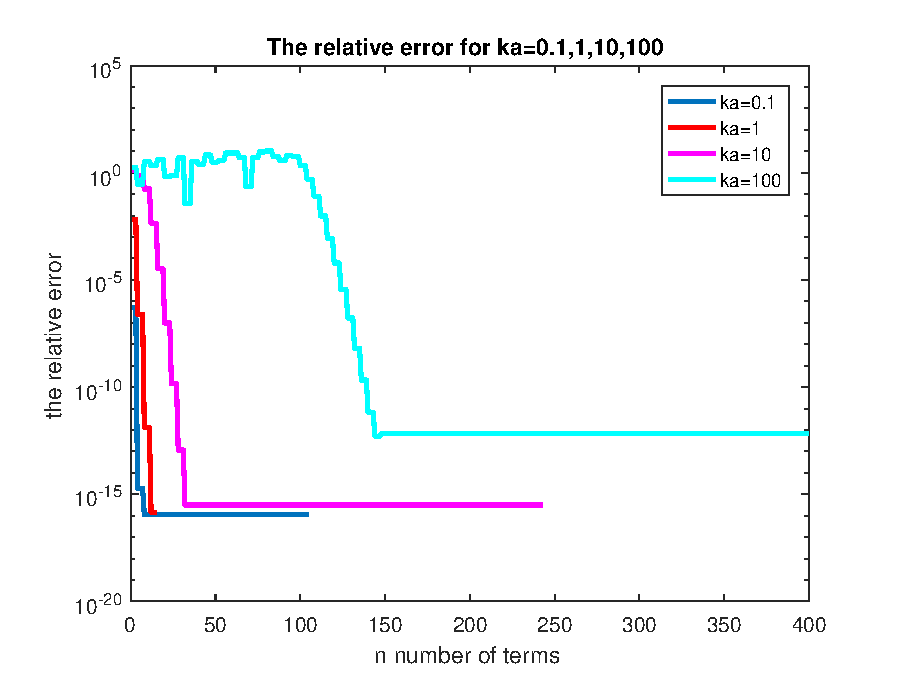
\includegraphics[scale=0.7]{ScatRelative}   
  \caption{The relative error calculated at $\rho=a$ for $ka=0.1,1,10,100$ at each order of Bessel function expansion.}           
\end{figure}
\\
Based on the relative error plotted in figure 1, for $ka=0.1$ and $ka=1$ roughly 10 terms is enough to compute the scattered field with a good accuracy, for $ka=10$ around 40 terms required and finally for $ka=100$ around 150 terms required.

\subsection*{c}
Plot (in MATLAB) the bistatic radar cross section of the cylinder for the four $ka$ values given in (b). That is, plot $RCS/\lambda$ (in dB) versus $\varphi$.
\\
\textbf{Solution:}\\
RCS in the far field is defined as: 
\begin{equation}
\label{eq:9}
\sigma = lim_{k\rho \rightarrow \infty} 2\pi \rho \frac{\left | \bar{E}_{scat}  \right |^2}{\left | \bar{E}_{inc} \right |^2}=\frac{16}{k}\left |\sum_{n=1}^{\infty} \frac{J_n(ka)}{H^{(2)}_n(ka)} \cos n(\phi-\phi_i) \right |^2
\end{equation}
\begin{figure}[!h]
    \centering
    \begin{subfigure}[b]{0.45\textwidth}
        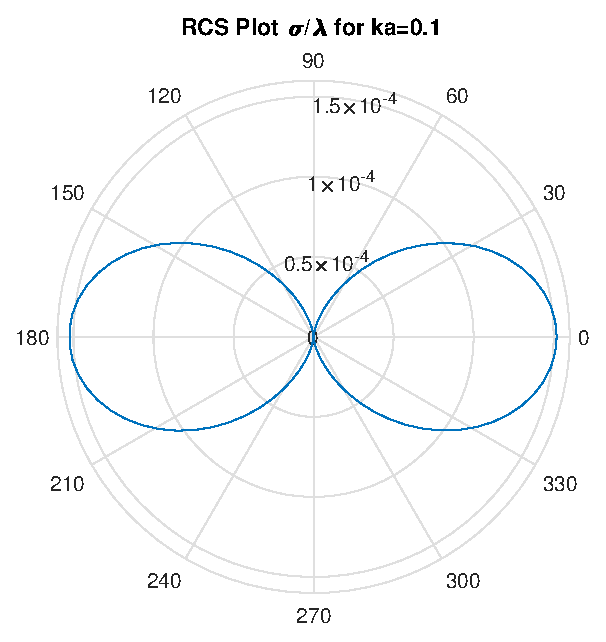
\includegraphics[width=\textwidth]{RCSka01}
        \caption{$ka=0.1$}
        \label{fig:gull}
    \end{subfigure}
    ~ %add desired spacing between images, e. g. ~, \quad, \qquad, \hfill etc. 
      %(or a blank line to force the subfigure onto a new line)
    \begin{subfigure}[b]{0.45\textwidth}
        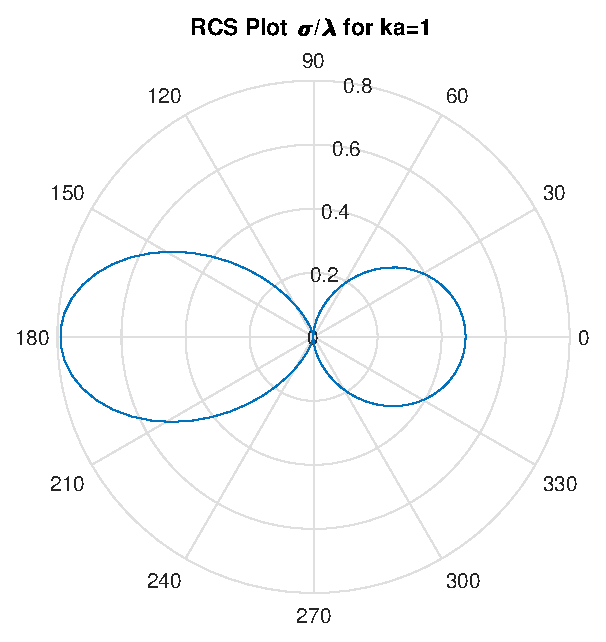
\includegraphics[width=\textwidth]{RCSka1}
        \caption{$ka=1$}
        \label{fig:tiger}
    \end{subfigure}
  \\
  \begin{subfigure}[b]{0.45\textwidth}
        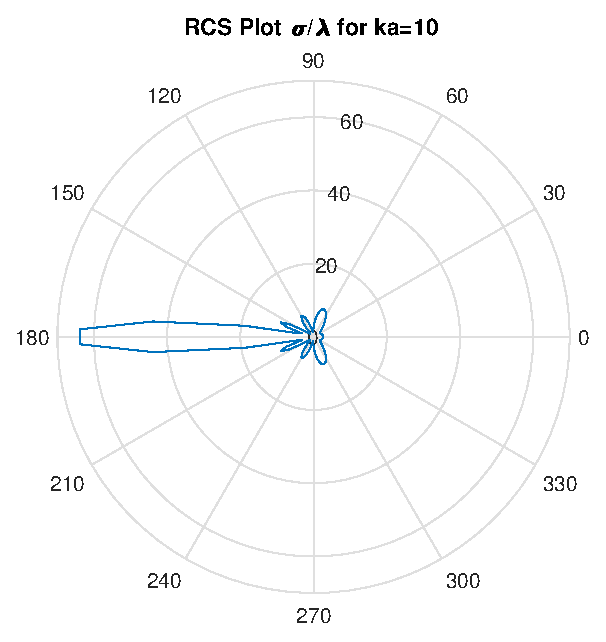
\includegraphics[width=\textwidth]{RCSka10}
        \caption{$ka=10$}
        \label{fig:gull}
    \end{subfigure}
    ~ %add desired spacing between images, e. g. ~, \quad, \qquad, \hfill etc. 
      %(or a blank line to force the subfigure onto a new line)
    \begin{subfigure}[b]{0.45\textwidth}
        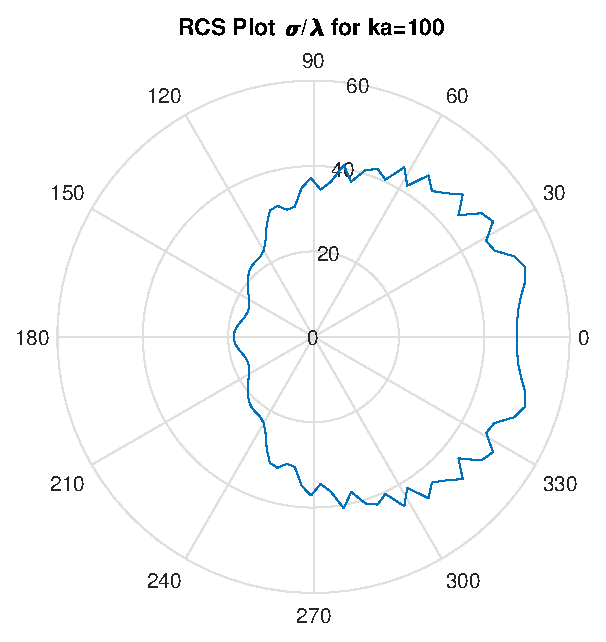
\includegraphics[width=\textwidth]{RCSka100}
        \caption{$ka=100$}
        \label{fig:tiger}
    \end{subfigure}
    \caption{RCS Plots}\label{fig:RCS}
\end{figure}
\newpage
\subsection*{d}
For this configuration and for the same incident field $E_{inc}(x)=e^{jkx}\hat{a}_z$, evaluate the
scattered far-field by the Physical Optics (PO) approach . If you are unable to evaluate
the PO integral analytically, use MATLAB to evaluate the integral numerically by $-\frac{\pi}{2}< \varphi' <\frac{\pi}{2}$ (the illuminated part of the cylinder). After obtaining the far-field expression of the scattered field $E_z(\bar{r})$ and the bistatic radar cross section of the cylinder with respect to $-\frac{\pi}{2}< \varphi' <\frac{\pi}{2}$ in dB scale for the following cases:
\begin{itemize}
\item $ka=10$
\item $ka=100$
\end{itemize}
Compare your results with those obtained by the analytical solution (i.e. the Mie series).
\\
\textbf{Solution:}\\
The incident $TM_x$ mode electric field inside the wave guide is given as:
\begin{equation}
\label{eq:10}
\begin{split}
\bar{E}_{inc}(\bar{r})=e^{-j k \rho \cos (\phi-\phi_i) }\hat{a}_z
\end{split}
\end{equation}
Corresponding magnetic field can be found by using the relation $\bar{\nabla}\times \bar{E}=-j\omega \bar{H}/\mu_0$, the magnetic field can be found as:
\begin{equation}
\label{eq:11}
\bar{H}_{inc}(\bar{r})=\frac{\omega k \sin(\phi-\phi_i)}{\mu_0 }e^{-j k \rho \cos (\phi-\phi_i) }\hat{a}_{\rho}-\frac{\omega k \cos(\phi-\phi_i)}{\mu_0 }e^{-j k \rho \cos (\phi-\phi_i) }\hat{a}_{\phi}
\end{equation}
By using the equivalence theorem, the equivalent surface electric current can be calculated as:
\begin{equation}
\bar{J}_s \approx 2\hat{a}_{\rho}\times \bar{H}_{inc}(\bar{a}) .
\end{equation}
As a result, the equivalent electric current at PEC surface is found as:
\begin{equation}
\bar{J}_s \approx \frac{2\omega k \cos(\phi-\phi_i)}{\mu_0 }e^{-j k \rho \cos (\phi-\phi_i) }\hat{a}_{z}
\end{equation}
The scattered electric field at the far field can be computed as:
\begin{equation}
\label{eq:12}
\bar{E}_{scat}(\bar{r})=-\frac{k \eta}{4 }\int \bar{J}_s(\bar{r}')H_{0}^{(2)}(k\left | \bar{r}-\bar{r}' \right |)a \mathrm{d} \phi \approx -\frac{k \eta}{4 }\sqrt{\frac{2j}{ \pi k r}}\int \bar{J}_s(\bar{r}') e^{-jk\left | \bar{r}-\bar{r}' \right |}a \mathrm{d} \phi.
\end{equation}
The integral in equation \ref{eq:12} can be explicitly given as:
\begin{equation}
\label{eq:13}
\bar{E}_{scat}(r,\phi) \approx -\frac{a \omega k^2 \eta }{2\mu_0 }\sqrt{\frac{2j}{ \pi k r}} \int_{-\pi/2}^{\pi/2} \cos(\phi'-\phi_i) e^{-j k a\cos (\phi'-\phi_i) }e^{-jk\sqrt{(r \cos\phi -a\cos \phi')^2+(r \sin\phi -a \sin \phi')^2}} \mathrm{d} \phi'.
\end{equation}
The integral \ref{eq:13} is taken numerically by trapezoidal rule for $-\pi/2 < \phi' < \pi/2$. The resultant electric field is compared with the electric field obtained by the series solution.
\newpage
\begin{figure}[!h]
    \centering
    \begin{subfigure}[b]{0.5\textwidth}
        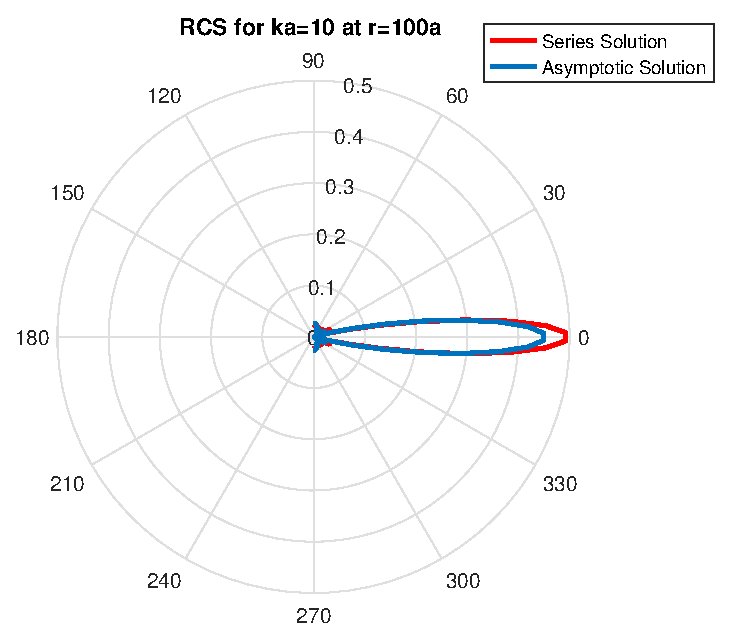
\includegraphics[width=\textwidth]{AsymRCSka10}
        \caption{RCS value for $ka=10$}
        \label{fig:gull}
    \end{subfigure}
    ~ %add desired spacing between images, e. g. ~, \quad, \qquad, \hfill etc. 
      %(or a blank line to force the subfigure onto a new line)
    \begin{subfigure}[b]{0.5\textwidth}
        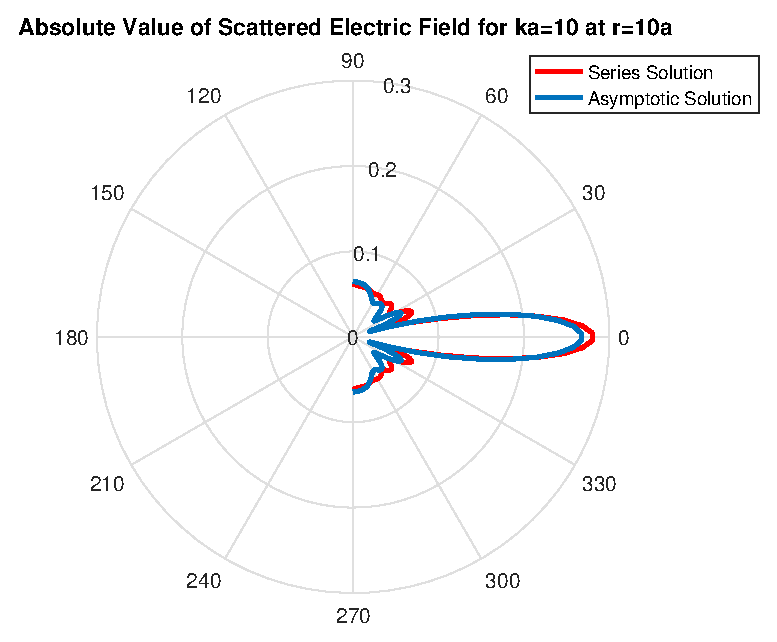
\includegraphics[width=\textwidth]{AsymEka10}
        \caption{Scattered Electric Field for $ka=10$}
        \label{fig:tiger}
    \end{subfigure}
  \\
  \begin{subfigure}[b]{0.5\textwidth}
        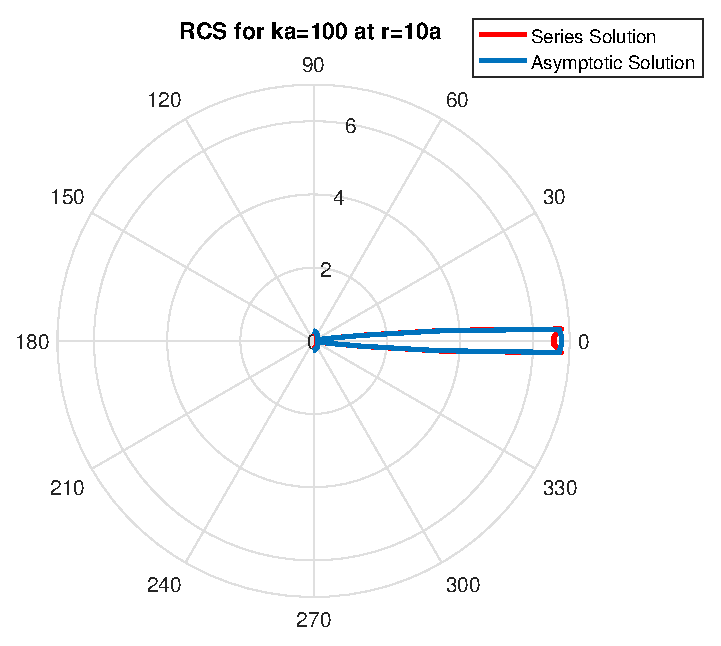
\includegraphics[width=\textwidth]{AsymRCSka100}
         \caption{RCS value for $ka=100$}
        \label{fig:gull}
    \end{subfigure}
    ~ %add desired spacing between images, e. g. ~, \quad, \qquad, \hfill etc. 
      %(or a blank line to force the subfigure onto a new line)
    \begin{subfigure}[b]{0.5\textwidth}
        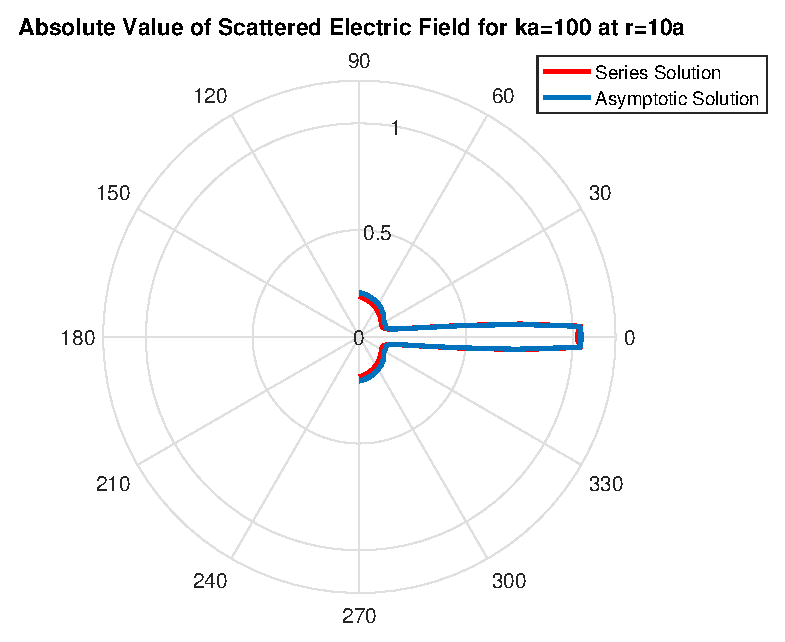
\includegraphics[width=\textwidth]{AsymEka100}
         \caption{Scattered Electric Field for $ka=100$}
        \label{fig:tiger}
    \end{subfigure}
    \caption{RCS Plots}\label{fig:RCS}
\end{figure}

\newpage

\appendix
\section{Matlab Codes}
\lstinputlisting[caption={Take Home Final Main Script}]{EE523TakeHomeFinal.m}
\lstinputlisting[caption={Bessel Junction Series Matlab Code}]{fun_cylinder_PEC.m}
\lstinputlisting[caption={RCS Plot Script}]{RCSPlot.m}
\lstinputlisting[caption={RCS Matlab Code}]{getRCS.m}
\lstinputlisting[caption={Asymptotic Electric Field Matlab Code}]{AsymptoticElectricField.m}
\lstinputlisting[caption={Asymptotic Electric Field Integration Matlab Code}]{getAysmptoticElectric.m}
\lstinputlisting[caption={Function Inside Integration Matlab Code}]{getIntFunc.m}
\end{document}
